\documentclass[11pt,]{article}
\usepackage[]{mathpazo}
\usepackage{amssymb,amsmath}
\usepackage{ifxetex,ifluatex}
\usepackage{fixltx2e} % provides \textsubscript
\ifnum 0\ifxetex 1\fi\ifluatex 1\fi=0 % if pdftex
  \usepackage[T1]{fontenc}
  \usepackage[utf8]{inputenc}
\else % if luatex or xelatex
  \ifxetex
    \usepackage{mathspec}
  \else
    \usepackage{fontspec}
  \fi
  \defaultfontfeatures{Ligatures=TeX,Scale=MatchLowercase}
\fi
% use upquote if available, for straight quotes in verbatim environments
\IfFileExists{upquote.sty}{\usepackage{upquote}}{}
% use microtype if available
\IfFileExists{microtype.sty}{%
\usepackage{microtype}
\UseMicrotypeSet[protrusion]{basicmath} % disable protrusion for tt fonts
}{}
\usepackage[margin=1in]{geometry}
\usepackage{hyperref}
\hypersetup{unicode=true,
            pdftitle={Case Study Elections Netherlands},
            pdfauthor={Ilse van Beelen and Floor Komen},
            pdfkeywords={put some keywords here},
            pdfborder={0 0 0},
            breaklinks=true}
\urlstyle{same}  % don't use monospace font for urls
\usepackage{natbib}
\bibliographystyle{plainnat}
\usepackage{color}
\usepackage{fancyvrb}
\newcommand{\VerbBar}{|}
\newcommand{\VERB}{\Verb[commandchars=\\\{\}]}
\DefineVerbatimEnvironment{Highlighting}{Verbatim}{commandchars=\\\{\}}
% Add ',fontsize=\small' for more characters per line
\usepackage{framed}
\definecolor{shadecolor}{RGB}{248,248,248}
\newenvironment{Shaded}{\begin{snugshade}}{\end{snugshade}}
\newcommand{\KeywordTok}[1]{\textcolor[rgb]{0.13,0.29,0.53}{\textbf{#1}}}
\newcommand{\DataTypeTok}[1]{\textcolor[rgb]{0.13,0.29,0.53}{#1}}
\newcommand{\DecValTok}[1]{\textcolor[rgb]{0.00,0.00,0.81}{#1}}
\newcommand{\BaseNTok}[1]{\textcolor[rgb]{0.00,0.00,0.81}{#1}}
\newcommand{\FloatTok}[1]{\textcolor[rgb]{0.00,0.00,0.81}{#1}}
\newcommand{\ConstantTok}[1]{\textcolor[rgb]{0.00,0.00,0.00}{#1}}
\newcommand{\CharTok}[1]{\textcolor[rgb]{0.31,0.60,0.02}{#1}}
\newcommand{\SpecialCharTok}[1]{\textcolor[rgb]{0.00,0.00,0.00}{#1}}
\newcommand{\StringTok}[1]{\textcolor[rgb]{0.31,0.60,0.02}{#1}}
\newcommand{\VerbatimStringTok}[1]{\textcolor[rgb]{0.31,0.60,0.02}{#1}}
\newcommand{\SpecialStringTok}[1]{\textcolor[rgb]{0.31,0.60,0.02}{#1}}
\newcommand{\ImportTok}[1]{#1}
\newcommand{\CommentTok}[1]{\textcolor[rgb]{0.56,0.35,0.01}{\textit{#1}}}
\newcommand{\DocumentationTok}[1]{\textcolor[rgb]{0.56,0.35,0.01}{\textbf{\textit{#1}}}}
\newcommand{\AnnotationTok}[1]{\textcolor[rgb]{0.56,0.35,0.01}{\textbf{\textit{#1}}}}
\newcommand{\CommentVarTok}[1]{\textcolor[rgb]{0.56,0.35,0.01}{\textbf{\textit{#1}}}}
\newcommand{\OtherTok}[1]{\textcolor[rgb]{0.56,0.35,0.01}{#1}}
\newcommand{\FunctionTok}[1]{\textcolor[rgb]{0.00,0.00,0.00}{#1}}
\newcommand{\VariableTok}[1]{\textcolor[rgb]{0.00,0.00,0.00}{#1}}
\newcommand{\ControlFlowTok}[1]{\textcolor[rgb]{0.13,0.29,0.53}{\textbf{#1}}}
\newcommand{\OperatorTok}[1]{\textcolor[rgb]{0.81,0.36,0.00}{\textbf{#1}}}
\newcommand{\BuiltInTok}[1]{#1}
\newcommand{\ExtensionTok}[1]{#1}
\newcommand{\PreprocessorTok}[1]{\textcolor[rgb]{0.56,0.35,0.01}{\textit{#1}}}
\newcommand{\AttributeTok}[1]{\textcolor[rgb]{0.77,0.63,0.00}{#1}}
\newcommand{\RegionMarkerTok}[1]{#1}
\newcommand{\InformationTok}[1]{\textcolor[rgb]{0.56,0.35,0.01}{\textbf{\textit{#1}}}}
\newcommand{\WarningTok}[1]{\textcolor[rgb]{0.56,0.35,0.01}{\textbf{\textit{#1}}}}
\newcommand{\AlertTok}[1]{\textcolor[rgb]{0.94,0.16,0.16}{#1}}
\newcommand{\ErrorTok}[1]{\textcolor[rgb]{0.64,0.00,0.00}{\textbf{#1}}}
\newcommand{\NormalTok}[1]{#1}
\usepackage{graphicx,grffile}
\makeatletter
\def\maxwidth{\ifdim\Gin@nat@width>\linewidth\linewidth\else\Gin@nat@width\fi}
\def\maxheight{\ifdim\Gin@nat@height>\textheight\textheight\else\Gin@nat@height\fi}
\makeatother
% Scale images if necessary, so that they will not overflow the page
% margins by default, and it is still possible to overwrite the defaults
% using explicit options in \includegraphics[width, height, ...]{}
\setkeys{Gin}{width=\maxwidth,height=\maxheight,keepaspectratio}
\IfFileExists{parskip.sty}{%
\usepackage{parskip}
}{% else
\setlength{\parindent}{0pt}
\setlength{\parskip}{6pt plus 2pt minus 1pt}
}
\setlength{\emergencystretch}{3em}  % prevent overfull lines
\providecommand{\tightlist}{%
  \setlength{\itemsep}{0pt}\setlength{\parskip}{0pt}}
\setcounter{secnumdepth}{0}
% Redefines (sub)paragraphs to behave more like sections
\ifx\paragraph\undefined\else
\let\oldparagraph\paragraph
\renewcommand{\paragraph}[1]{\oldparagraph{#1}\mbox{}}
\fi
\ifx\subparagraph\undefined\else
\let\oldsubparagraph\subparagraph
\renewcommand{\subparagraph}[1]{\oldsubparagraph{#1}\mbox{}}
\fi

%%% Use protect on footnotes to avoid problems with footnotes in titles
\let\rmarkdownfootnote\footnote%
\def\footnote{\protect\rmarkdownfootnote}

%%% Change title format to be more compact
\usepackage{titling}

% Create subtitle command for use in maketitle
\newcommand{\subtitle}[1]{
  \posttitle{
    \begin{center}\large#1\end{center}
    }
}

\setlength{\droptitle}{-2em}

  \title{Case Study Elections Netherlands}
    \pretitle{\vspace{\droptitle}\centering\huge}
  \posttitle{\par}
    \author{Ilse van Beelen and Floor Komen}
    \preauthor{\centering\large\emph}
  \postauthor{\par}
      \predate{\centering\large\emph}
  \postdate{\par}
    \date{december 21, 2018}

\usepackage{booktabs}
\usepackage{longtable}
\usepackage{array}
\usepackage{multirow}
\usepackage[table]{xcolor}
\usepackage{wrapfig}
\usepackage{float}
\usepackage{colortbl}
\usepackage{pdflscape}
\usepackage{tabu}
\usepackage{threeparttable}
\usepackage{threeparttablex}
\usepackage[normalem]{ulem}
\usepackage{makecell}

\usepackage{float}

\begin{document}
\maketitle
\begin{abstract}
Put the abstract over here
\end{abstract}

\section{1. Introduction}\label{introduction}

In this report the election

\subsection{1.1 Motivation}\label{motivation}

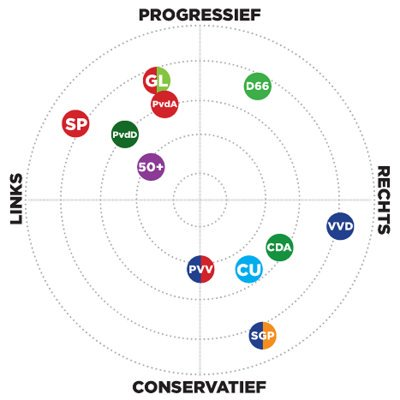
\includegraphics[width=2.60417in]{Partijlandschap.jpg} \textbf{Dutch
political parties}\\
In this landscape the diffence between the parties is graphically
displayed in this figure. In this research, two parties are chosen to
investigate. These two parties had to be different, so that some
comparisons could be made. The parties should not be to extreme
left/right/conservative/progressive, so that the model will be proven to
work on less-extreme parties. Therefore, the chosen parties are: CDA and
GroenLinks. After the data-cleaning the CDA will be researched first,
afterwards GroenLinks will be researched.

In this research the above described demographics are chosen because of
there influence on a municipality level. The thought is that a more
non-western municipality for example votes different than a less
non-western municipality. This is the same for the other two
demographics. Other demographics are also researched, for example
gender, but on a municipality level there is no big difference between
the amount of men and women per municipality. So that is a more
interesting demographic to research on an individual level. \emph{The
standardized income per municipality} are given in thousands. \emph{the
urban index of a municipality} is a database with five categories per
municipality. These five categories are; really strong urban (more than
2500 addresses per km2), strong urban (1500-2500 addresses per km2),
moderate urban (1000- 1500 addresses per km2), little urban (500-1000
addresses per km2) and not urban (less than 500 addresses per km2). Per
municipality the amount of km2 per category is given. The \emph{non-west
residents per municipality} is given in an amount per municipality, also
the total amount of residents is given per municipality.

\subsection{1.2 Data sources}\label{data-sources}

\textbf{Electoral data} For the electoral data we used the results of
the 2017 general election. This is the most recent national election and
is of the most important election type. Therefore, it seems plausible
that the data for this election is representative of the political
makeup of different municipalities. We downloaded the raw data directly
from the official government source.\footnote{\url{https://data.overheid.nl/data/dataset/verkiezingsuitslag-tweede-kamer-2017}}
This contained a .csv file with the raw number of votes for every party
in every municipality.

\textbf{Demographical data}\\
We got our demographical data from the CBS, the official Dutch
statistical agency.\footnote{\url{https://opendata.cbs.nl/statline/\#/CBS/nl/dataset/70072ned/table?ts=1544803364892}}
From the wealth of demographical information available we picked a
handful of attributes that we suspected (based on prior research and
some gut feeling) to be useful as predictor variables. We landed on five
demographical attributes: education grade, average income, age,
urbanization and the amount of people with a non-western background.
Note that the data we downloaded from the CBS site usually had to be
transformed to get it in a useful predictor variable format. The
specifics of this are described in the next section.

\subsection{1.3 Data cleaning}\label{data-cleaning}

The data cleaning is the process in which we used

\textbf{Electoral data}

\textbf{Demographical data}

The variable \emph{non-western residents} are divided in three groups.
Municipalities with less than 5 \% non-western residents, 5-10 \%
non-western residents and municipalities with more dan 10 \% non-western
residents.

\begin{Shaded}
\begin{Highlighting}[]
\NormalTok{Data <-}\StringTok{ }\KeywordTok{read.csv}\NormalTok{(}\StringTok{"1_clean_data/voting_and_demographics.csv"}\NormalTok{, }\DataTypeTok{stringsAsFactors =}\NormalTok{ F, }
    \DataTypeTok{header =}\NormalTok{ T)}
\NormalTok{Data <-}\StringTok{ }\NormalTok{Data[, }\OperatorTok{-}\DecValTok{15}\NormalTok{]}
\KeywordTok{colnames}\NormalTok{(Data) <-}\StringTok{ }\KeywordTok{c}\NormalTok{(}\StringTok{"Muni"}\NormalTok{, }\StringTok{"VVD"}\NormalTok{, }\StringTok{"CDA"}\NormalTok{, }\StringTok{"PVV"}\NormalTok{, }\StringTok{"D66"}\NormalTok{, }\StringTok{"SP"}\NormalTok{, }\StringTok{"GL"}\NormalTok{, }\StringTok{"PvdA"}\NormalTok{, }
    \StringTok{"CU"}\NormalTok{, }\StringTok{"50PLUS"}\NormalTok{, }\StringTok{"PvdD"}\NormalTok{, }\StringTok{"SGP"}\NormalTok{, }\StringTok{"FvD"}\NormalTok{, }\StringTok{"DENK"}\NormalTok{, }\StringTok{"Urban_index"}\NormalTok{, }\StringTok{"High_edu_perc"}\NormalTok{, }
    \StringTok{"Mean_income"}\NormalTok{, }\StringTok{"Dutch_perc"}\NormalTok{, }\StringTok{"West_perc"}\NormalTok{, }\StringTok{"Non_west_perc"}\NormalTok{)}
\NormalTok{Data}\OperatorTok{$}\NormalTok{Non_west <-}\StringTok{ }\KeywordTok{ifelse}\NormalTok{(Data}\OperatorTok{$}\NormalTok{Non_west_perc }\OperatorTok{<}\StringTok{ }\FloatTok{0.05}\NormalTok{, }\DecValTok{1}\NormalTok{, }\OtherTok{NA}\NormalTok{)}
\NormalTok{Data}\OperatorTok{$}\NormalTok{Non_west <-}\StringTok{ }\KeywordTok{ifelse}\NormalTok{(Data}\OperatorTok{$}\NormalTok{Non_west_perc }\OperatorTok{>=}\StringTok{ }\FloatTok{0.05} \OperatorTok{&}\StringTok{ }\NormalTok{Data}\OperatorTok{$}\NormalTok{Non_west_perc }\OperatorTok{<}\StringTok{ }\FloatTok{0.1}\NormalTok{, }
    \DecValTok{2}\NormalTok{, Data}\OperatorTok{$}\NormalTok{Non_west)}
\NormalTok{Data}\OperatorTok{$}\NormalTok{Non_west <-}\StringTok{ }\KeywordTok{ifelse}\NormalTok{(Data}\OperatorTok{$}\NormalTok{Non_west_perc }\OperatorTok{>=}\StringTok{ }\FloatTok{0.1}\NormalTok{, }\DecValTok{3}\NormalTok{, Data}\OperatorTok{$}\NormalTok{Non_west)}
\NormalTok{Data}\OperatorTok{$}\NormalTok{Non_west <-}\StringTok{ }\KeywordTok{as.factor}\NormalTok{(Data}\OperatorTok{$}\NormalTok{Non_west)}
\NormalTok{Dat_cda <-}\StringTok{ }\NormalTok{Data[, }\KeywordTok{c}\NormalTok{(}\DecValTok{1}\NormalTok{, }\DecValTok{3}\NormalTok{, }\DecValTok{15}\NormalTok{, }\DecValTok{16}\NormalTok{, }\DecValTok{17}\NormalTok{, }\DecValTok{21}\NormalTok{)]}
\NormalTok{Dat_cda <-}\StringTok{ }\NormalTok{Dat_cda[}\KeywordTok{complete.cases}\NormalTok{(Dat_cda), ]}
\end{Highlighting}
\end{Shaded}

\subsection{1.3 Data visualisation}\label{data-visualisation}

In this part the cleaned data is visualized, so that a good picture can
be obtained of the current data. First of all some demographics of data
will be showed. In figure \ref{1} of the \emph{parties}, \emph{the urban
index}, \emph{the percentage of highly educated residents}, \emph{the
mean income}, \emph{The non west residents factor} and * the percentage
60 plus* are plotted. As you can see in the plot, they are normal
distributed. Because of the low values at the x-axis, the CDA,
GroenLinks, 60 plus percentage and the highly educated densities are
above 1. The area beneath the curve sums to 1, so it is correct.
\rowcolors{2}{gray!6}{white}

\begin{table}

\caption{\label{tab:demographics_data1}Data summary}
\centering
\resizebox{\linewidth}{!}{
\begin{tabular}[t]{llllllll}
\hiderowcolors
\toprule
  &      CDA &       GL &  Urban\_index & High\_edu\_perc &  Mean\_income &    Non\_west &  Perc\_60plus\\
\midrule
\showrowcolors
 & Min.   :0.031 & Min.   :0.0025 & Min.   :0.00 & Min.   :0.12 & Min.   :21 & Min.   :1.0 & Min.   :0.067\\
 & 1st Qu.:0.116 & 1st Qu.:0.0539 & 1st Qu.:0.66 & 1st Qu.:0.22 & 1st Qu.:24 & 1st Qu.:1.0 & 1st Qu.:0.123\\
 & Median :0.142 & Median :0.0657 & Median :1.22 & Median :0.26 & Median :26 & Median :2.0 & Median :0.134\\
 & Mean   :0.152 & Mean   :0.0714 & Mean   :1.43 & Mean   :0.27 & Mean   :26 & Mean   :1.7 & Mean   :0.133\\
 & 3rd Qu.:0.182 & 3rd Qu.:0.0846 & 3rd Qu.:2.18 & 3rd Qu.:0.30 & 3rd Qu.:27 & 3rd Qu.:2.0 & 3rd Qu.:0.142\\
 & Max.   :0.420 & Max.   :0.2055 & Max.   :3.79 & Max.   :0.53 & Max.   :42 & Max.   :3.0 & Max.   :0.178\\
\bottomrule
\end{tabular}}
\end{table}

\rowcolors{2}{white}{white}

\begin{figure}[H]

{\centering 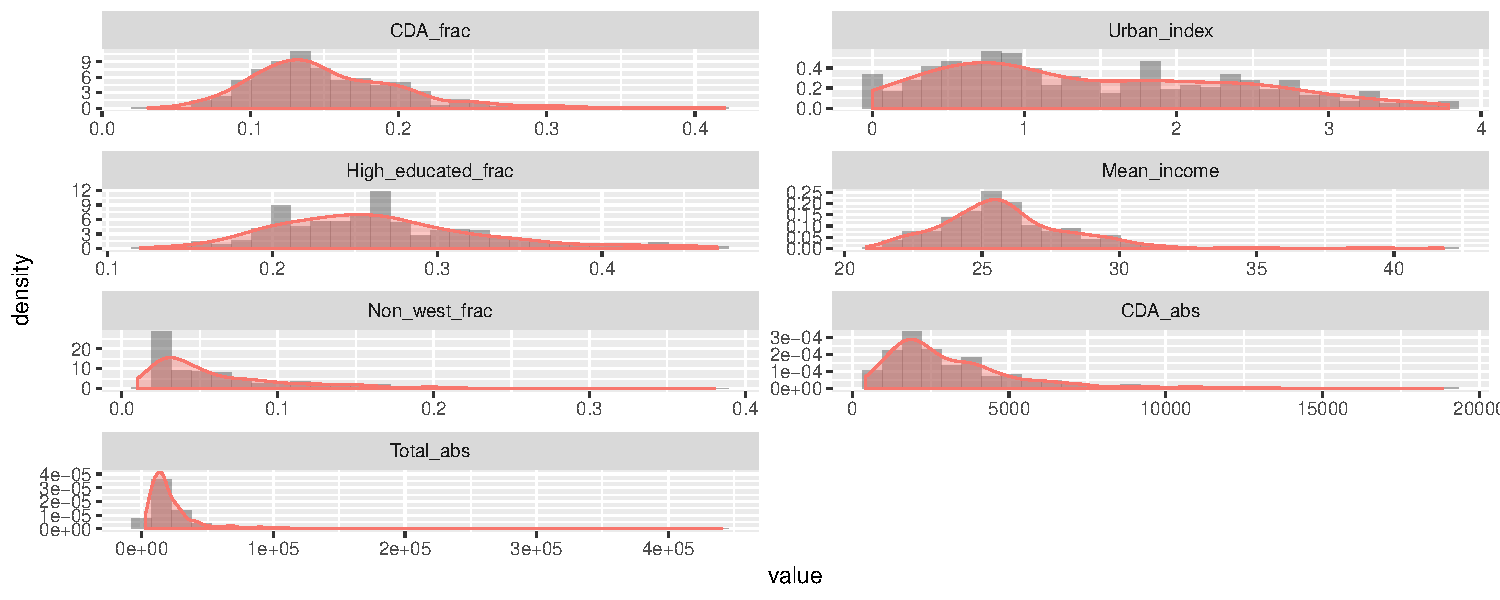
\includegraphics{Report_files/figure-latex/demographics_data-1} 

}

\caption{\label{1} Density plot}\label{fig:demographics_data}
\end{figure}

\textbf{Correlation heatmap} In this heatmap the correlation between
explanatory and respons variable are showed. The red color means a
positive relation, the purple color means a negative relation. The
non\_west variable is not taken into account, because it is a factor and
the other variables are continous. VERDER UITLEG

\begin{figure}[H]

{\centering 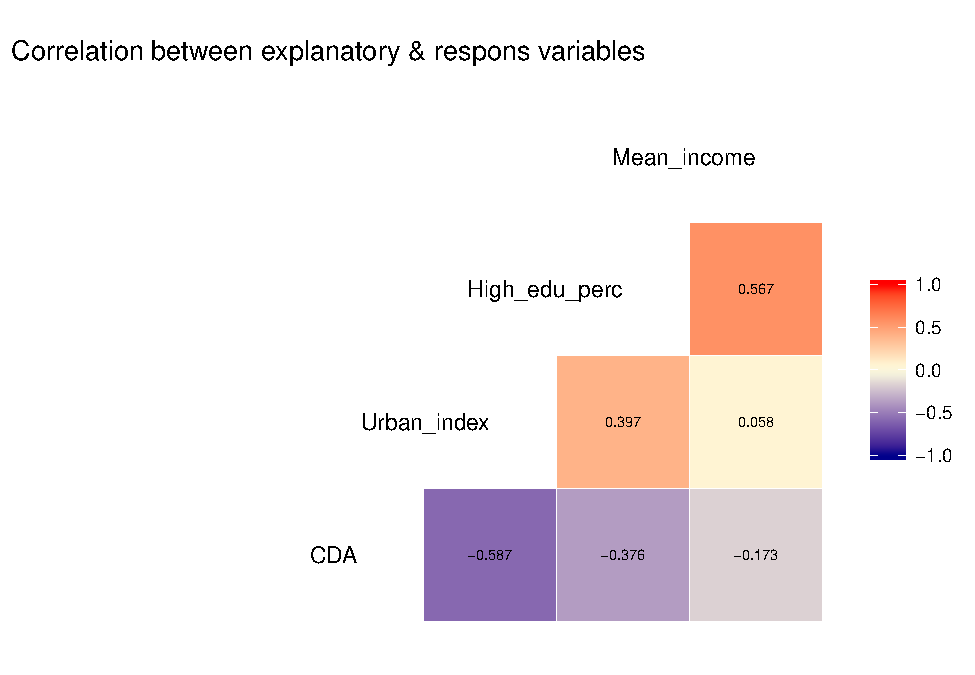
\includegraphics{Report_files/figure-latex/correlation_heatmap-1} 

}

\caption{Correlation between explanatory and respons variables}\label{fig:correlation_heatmap}
\end{figure}

\textbf{Multilineair plots CDA } In these two plots you can see a
scatterplot with on the y-axis the votes for CDA in percentages and on
the x-axis on the left graph the mean income per municipality in 1000
euro. The right plot has the urbanity index as x-axis. As you can see,
the trend is that when the mean income goes up, the votes for CDA goes
down. Same with the urbanity index. In the model formulation graph these
trends are checked.

\begin{figure}[H]

{\centering 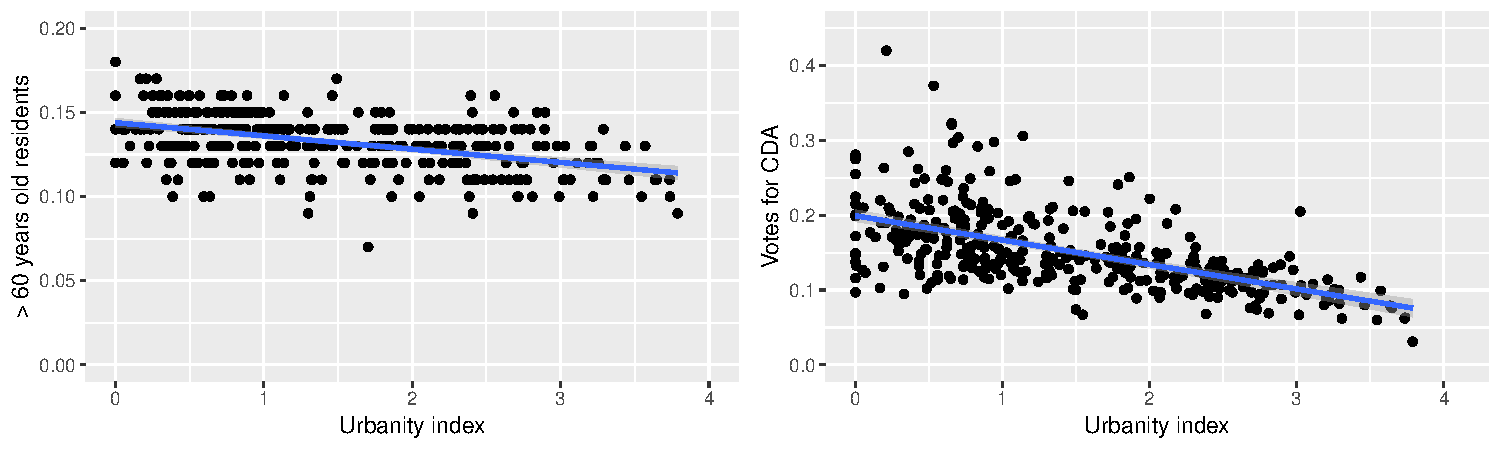
\includegraphics{Report_files/figure-latex/unnamed-chunk-5-1} 

}

\caption{Scatterplots CDA}\label{fig:unnamed-chunk-5}
\end{figure}

\textbf{Multilineair plots Groenlinks}

In these plots the percentage of votes for GL are compared with urbanity
index and percentage of highly educated residents. When municipalities
get more crowded, the trend is that votes for GL goes up. The other
visible trend is that when more residents in a municipality are highly
educated, GL got more votes.\\

\begin{figure}[H]

{\centering 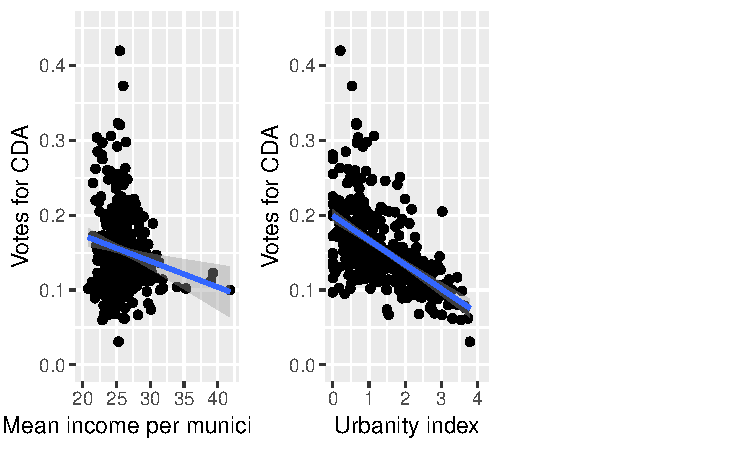
\includegraphics{Report_files/figure-latex/unnamed-chunk-6-1} 

}

\caption{Scatterplot GroenLinks}\label{fig:unnamed-chunk-6}
\end{figure}

\textbf{Multilinear plots explanatory variables} These three plots are
scatterplots about explanatory variables.

\begin{figure}[H]

{\centering 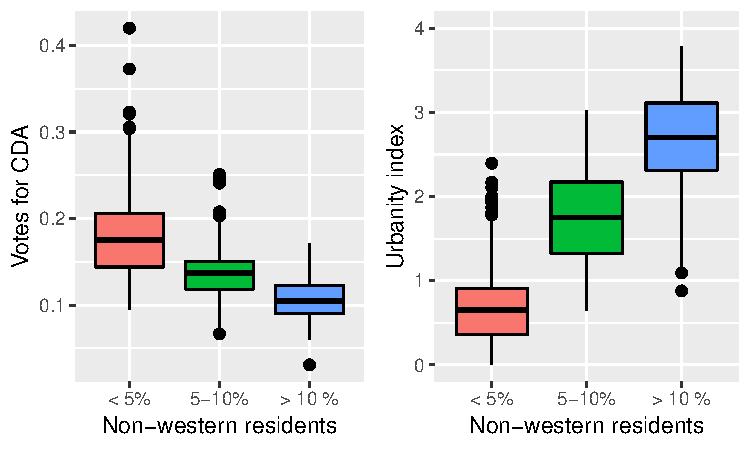
\includegraphics{Report_files/figure-latex/unnamed-chunk-7-1} 

}

\caption{Scatterplot explanatory variables}\label{fig:unnamed-chunk-7}
\end{figure}

\textbf{Multiple boxplots} In this graph boxplots are made, to compare
some variables. A boxplot is a standardized way to display the
distribution of data. It gives the minimum, first quartile, median,
third quartile and the maximum. If there are any outliers, the boxplot
is extended with those. The line within the box is the median, the first
and third quartile are the down- and upside of the box. The length of
the box is the Inter Quartile Range (IQR). The minimum and maximum are
1.5XIQR distance. Outliers are thus further away than 1.5XIQR.

\begin{figure}[H]

{\centering 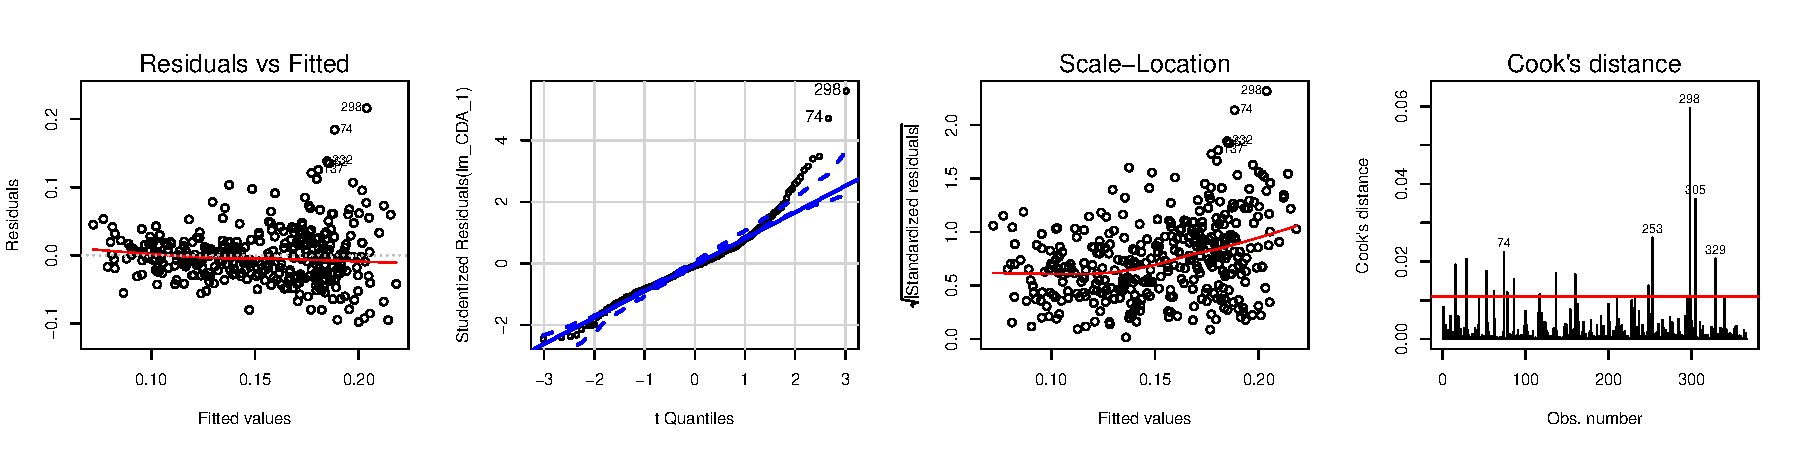
\includegraphics{Report_files/figure-latex/unnamed-chunk-8-1} 

}

\caption{Three boxplots: Votes for CDA, Votes for GroenLinks and Urbanity index}\label{fig:unnamed-chunk-8}
\end{figure}

\section{2. Formulate model}\label{formulate-model}

Model formuleren

\subsection{CDA}\label{cda}

\subsection{GroenLinks}\label{groenlinks}

\section{3 Final model}\label{final-model}

\subsection{CDA}\label{cda-1}

\subsection{Groenlinks}\label{groenlinks-1}

\section{4 Analyse output}\label{analyse-output}

\section{5 Discussion}\label{discussion}

\subsection{5.1 Limitations}\label{limitations}


\end{document}
